
\chapter[Design Flow for SMC Applications]{Design Flow for Sequential Monte Carlo Applications}

%%%%%%%%%%%%%%%%%%%%%%%%%%%%%%%%%%%%%%%%%%%%%%%%%%%%%%%%%%%%%%%
\section{Introduction}
\label{sec:intro}

Sequential Monte Carlo (SMC) methods are a set of on-line posterior density estimation algorithms that perform inference of unknown quantities from observations.
The observations arrive sequentially in time and the inference is performed on-line.
A common application is in the guidance, navigation and control of vehicles, particularly mobile robots~\cite{montemerlo02} and aircraft~\cite{kantas09}.
For these applications, it is critical that high sampling rates can be handled in real-time.
SMC methods also have applications in economics and finance~\cite{creal12} where minimising latency is crucial.
 
SMC methods are often preferable to Kalman filters and hidden Markov models, as they do not require exact analytical expressions to compute the evolving sequence of posterior distributions.
Moreover, they can model high-dimensional data using non-linear dynamics and constraints, are parallelisable, and can greatly benefit from hardware acceleration.
Acceleration of SMC methods has been studied in applications such as air traffic management~\cite{chau13b,eele13}, robot localisation~\cite{chau13a}, object tracking~\cite{happe13} and signal processing~\cite{hendeby07}.

While SMC has been implemented efficiently on FPGAs~\cite{chau13a,chau13b,happe13,hendeby07}, design productivity remains a challenge.
Firstly, while different sets of SMC parameters produce the same accuracy, they have very different computational complexity.
For example, the performance of SMC relies on a set of random samples, which are called particles in the following.
The more complex the problem, the larger the number of particles needed.
Using excessive numbers of particles unfortunately causes prohibitive run-time without increasing solution accuracy.
The parameter space spans multiple dimensions and the objective function can be non-convex, making exhaustive optimisation impractical.
Secondly, customising designs for different SMC applications requires tremendous effort.

In this chapter, we propose an SMC design flow for reconfigurable hardware.
A computation engine captures the generic control structure shared among all SMC applications.
A framework for mapping software to hardware is derived, so users can specify application-specific features which are automatically converted to efficient hardware. 
Timing model relates design parameters to performance constraints.
To enable rapid learning of a large design space, a machine learning algorithm is used to automatically deduce characteristics of the design space.

The contributions are as follows:
\begin{itemize}
\item A design flow to reduce the development effort of SMC applications on reconfigurable systems (Section~\ref{sec:design}). Through templating the SMC structure, users can design efficient, multiple-FPGA SMC applications for arbitrary problems without any knowledge of reconfigurable computing, and the software template is open-source.\footnote{Available online: \url{http://cc.doc.ic.ac.uk/projects/smcgen}}
\item A machine learning approach that explores the SMC design space automatically and tunes design parameters to improve performance and accuracy (Section~\ref{sec:optimisation}). The resulting parameters can be applied to the hardware design at run-time without the need for resynthesis.
It is demonstrated that parameter optimisation enables the design space to be explored an order of magnitude faster without sacrificing quality.
Compared with previous work~\cite{chau13a,chau13b}, we have achieved better quality of solutions and faster designs.
\item The benefitbenefit  of this approach in terms of design productivity and performance is quantified over a diverse set of SMC problems.
Three applications are implemented on Altera and Xilinx-based reconfigurable platforms, with varying numbers of FPGAs. For these problems, the number of lines of code for the FPGA implementation is reduced by approximately 76\%, and 
significant speedup and energy improvement over CPU and GPU implementations (Section~\ref{sec:evaluation}) are demonstrated.
\end{itemize}


%%%%%%%%%%%%%%%%%%%%%%%%%%%%%%%%%%%%%%%%%%%%%%%%%%%%%%%%%%%%%%%
\section{Overview}
\label{sec:overview}

\subsection{SMC Methods}
\label{sec:smc}

SMC methods estimate the unobserved states of interest based on observations in controlling various agents~\cite{doucet01}.
The target posterior density $p(s_t|m_t)$ is represented by a set of particles, where $s_t$ is the state and $m_t$ is the observation at time step $t$.
A sequential importance resampling (SIR) algorithm~\cite{gordon93} is used to obtain a weighted set of $N_P$ particles $\{s_t^{(i)},w_t^{(i)}\}^{N_P}_{i=1}$.
The importance weights $\{w_t^{(i)}\}^{N_P}_{i=1}$ are approximations to the relative posterior probabilities of the particles such that $\sum^{N_P}_{i=1}w^{(i)}_t = 1$.
This process is described in Algorithm~\ref{algo:smc} and involves five stages of computation:

\begin{algorithm}
\caption{SMC methods}
\footnotesize
\begin{algorithmic}[1]
\FOR {each time step t}
\STATE {$idx1 \gets 0$}
\STATE {Initialisation}
\WHILE {$idx1 \le itl\_outer$}
	\STATE {$idx2 \gets 0$}
	\STATE {$itl\_inner \gets 3+5\exp(\frac{5*idx1}{itl\_outer})$}
	\FOR {each particle p}
		\WHILE {$idx2 \le itl\_inner$}
			\STATE {Sampling} \label{algo:s}
			%\STATE {\hspace{\algorithmicindent}$\hookrightarrow$ Disturbance realisation}
			%\STATE {\hspace{\algorithmicindent}$\hookrightarrow$ Trajectory planning}
			\STATE {Importance weighting} \label{algo:i}
			%\STATE {\hspace{\algorithmicindent}$\hookrightarrow$ Score calculation}
			%\STATE {\hspace{\algorithmicindent}$\hookrightarrow$ Constraint handling}
			%\STATE {\hspace{\algorithmicindent}$\hookrightarrow$ Weight calculation and normalisation}
			\STATE {$idx2 \gets idx2+1$}
		\ENDWHILE
	\ENDFOR
	\STATE {$idx1 \gets idx1+1$}
	\IF {$idx1 \le itl\_inner$}
		\STATE {Resampling}
	\ENDIF
\ENDWHILE
\STATE {Update}
\ENDFOR
\end{algorithmic}
\label{algo:smc}
\end{algorithm}

\begin{enumerate}
\item \textbf{Initialisation}: Weights $\{w_t^{(i)}\}^{N_P}_{i=1}$ are set to $\frac{1}{N_P}$.
\item \textbf{Sampling}: Next states $\{s_t^{'(i)}\}^{N_P}_{i=1}$ are computed based on the current state $\{s_{t-1}^{(i)}\}^{N_P}_{i=1}$.
\item \textbf{Importance weighting}: Weight $\{w_t^{(i)}\}^{N_P}_{i=1}$ is updated based on a score function which accounts for the likelihood of particles fitting the observation.
Within each iteration $idx1$, the sampling and importance weighting stages are iterated $itl\_inner$ times so that those particles with sustained benefits are assigned higher weights.
As $idx1$ increases, the set of particles reflects a more accurate approximation, so $itl\_inner$ is increased exponentially.
\item \textbf{Resampling}: By removing the particles with small weights and replicating those with large weights
$itl\_outer$ times in a time step, the problem of degeneracy is addressed~\cite{kitagawa96}. Without this step, only a small number of particles will have substantial weights for inference.
\item \textbf{Update}: State $s_t$ is obtained from the resampled particle set $\{s_t^{(i)}\}^{N_P}_{i=1}$ via weighted average or more complicated functions that will be shown below.
\end{enumerate}

Table~\ref{tab:parameters} summarises the parameters of the SMC methods described in Section~\ref{sec:smc}.

\begin{table}
	\setlength{\tabcolsep}{3pt}
	\begin{spacing}{1.0}
	\caption{SMC design parameters. Dynamic: adjustable at run-time; static: fixed at compile-time.}
	\label{tab:parameters}
	\footnotesize
	\centering
	\smallskip
		\begin{tabular}{c|c|c}
			\hline
			 Parameters & Description & Type\\
			\hline
			\hline
			$itl\_outer$ & Number of iterations of the outer loop & \multirow{4}{*}{Dynamic}\\
			$itl\_inner$ & Number of iterations of the inner loop &\\
			$N_P$ & Number of particles &\\
			$S$ & Scaling factor for standard deviation of noise &\\
			\hline
			$H$ & Prediction horizon & \multirow{2}{*}{Static}\\
			$N_A$ & Number of agents under control &\\
			\hline
		\end{tabular}
		\end{spacing}
\end{table}


\subsection{SMC Applications}
\subsubsection{Stochastic Volatility}
\label{sec:vol}

These models are used extensively in mathematical
finance~\cite{casarin04,weng12}, and describe volatility as a
stochastic process which better reflects the behaviour of many
financial instruments but are computationally expensive. In this
work, the sampling function shown in Equation~\ref{eq:sv_model} is employed,
where $y_t$ is the observable time varying volatility and $s_t$ represents the stochastic log-volatility process.
$\beta$ and $\phi$ are empirical constants.

\begin{equation}
\footnotesize
\begin{aligned}
	y_t &= \beta \exp(s_t/2)\epsilon_t \mbox{, } \epsilon_t \sim \mathcal{N}(0,1) \\
	s_t &= \phi s_{t-1} + \mathcal{N}(0,1)
\end{aligned}
\label{eq:sv_model}
\end{equation}

The sampling function in Equation~\ref{eq:sv} is implied by Equation~\ref{eq:sv_model}.
The state transition from $s_{t-1}$ to $s_t$ is used to draw random samples $s^i_t$ from the existing pool of particles.

\begin{equation}
\footnotesize
\begin{aligned}
	s^i_{t} \sim \mathcal{N}(\phi s^i_{t-1},1)
\end{aligned}
\label{eq:sv}
\end{equation}

\subsubsection{Robot Localisation}
SMC methods are applied to mobile robot localisation~\cite{montemerlo02},
and this application is used as an example throughout the paper.
At regular time intervals, a robot obtains sensor values, identifies its location and commits a move.
The robot needs to be aware of the locations of other moving objects in the environment.

The sampling stage is described by Equations~\ref{eq:mcl_s} and~\ref{eq:mcl_r}. 
The robot estimates its updated state $s_t$ based on the current known location ($x, y$) and heading $h$.
State is affected by external reference status $r_t$ which contains displacement $\delta$ and rotation $\gamma$.
Importance weighting is used to calculate the likelihood of a location based on the observation, i.e. the sensor values.

\begin{equation}
\footnotesize
\begin{aligned}
  \begin{pmatrix}
    s^i_{t}    \\ 
  \end{pmatrix}
  =
  \begin{pmatrix}
    x^i_{t}    \\ 
    y^i_{t}    \\ 
    h^i_{t}    \\ 
  \end{pmatrix}
  =
  \begin{pmatrix}
  	x^i_{t-1} + \delta^{'i}_{t} \cos(h^i_{t-1}) \\
		y^i_{t-1} + \delta^{'i}_{t} \sin(h^i_{t-1}) \\
		h^i_{t-1} + \gamma^{'i}_{t} \\
  \end{pmatrix}
\end{aligned}
\label{eq:mcl_s}
\end{equation}

\begin{equation}
\footnotesize
\begin{aligned}
  \begin{pmatrix}
    r^i_{t}    \\ 
  \end{pmatrix}
  =
  \begin{pmatrix}
    \delta^{'i}_{t}    \\ 
    \gamma^{'i}_{t}    \\ 
  \end{pmatrix}
  =
  \begin{pmatrix}
  	\mathcal{N}(\delta_{t},\sigma_a^2) \\
		\mathcal{N}(\gamma_{t},\sigma_b^2) \\
  \end{pmatrix}
\end{aligned}
\label{eq:mcl_r}
\end{equation}


\subsubsection{Air Traffic Management}
\label{sec:atm}

SMC methods are applied to model predictive control (MPC) optimisation where control actions at discrete time intervals are determined to minimise error criteria~\cite{kantas09}.
An example is air traffic management which avoids dangerous encounters by maintaining safe separation distances between aircraft.
%The management system also seeks to improve the time of arrival of aircraft through minimising delays and unnecessary holding.

At each sampling instant, the control sequence over a number of future time steps, called the prediction horizon $H$, is estimated.
A state is a set of control sequences $\{s_t^{(i),0...H-1}\}^{N_P}_{i=1}$ being picked within a permitted range and applied to the current reference status $r_{t-1}$ to compute the future set of reference statuses $\{r_t^{'{(i),0...H-1}}\}^{N_P}_{i=1}$.
During importance weighting, a score function evaluates the quality of estimation for each particle, and weights the product of scores over the horizon.
If any particle violates any constraint, its weight is set to zero.
The first control $s_{t}^0$ in the sequence, is obtained by selecting the best one among $\{s_t^{(i),0...H-1}\}^{N_P}_{i=1}$.
Then the selected control is committed to form reference $r_t$.

Equation~\ref{eq:atm_c} illustrates a control tuple that consists of roll angle $\phi$; pitch angle $\tau$; and thrust $T$.
Equation~\ref{eq:atm_s} shows a reference that consists of the current position in 3 dimensional space $(x,y,a)$, heading angle $\chi$, air speed $V$ and mass $M$. 
For more details of the model, see~\cite{eele13}.

\begin{equation}
\footnotesize
\begin{aligned}
  \begin{pmatrix}
    s^i_{t}    \\ 
  \end{pmatrix}
  =
  \begin{pmatrix}
  	\phi^{'i}_{t} \\
		\tau^{'i}_{t} \\
		T^{'i}_{t} \\
  \end{pmatrix}
  =
  \begin{pmatrix}
  	\mathcal{N}(\phi_{t},\sigma_a^2) \\
  	\mathcal{N}(\tau_{t},\sigma_b^2) \\
  	\mathcal{N}(T_{t},\sigma_c^2) \\
  \end{pmatrix}
\end{aligned}
\label{eq:atm_c}
\end{equation}

\begin{equation}
\footnotesize
\begin{aligned}
  \begin{pmatrix}
    r^{'i}_{t}    \\ 
  \end{pmatrix}
  =
  \begin{pmatrix}
    x^i_{t}    \\ 
    y^i_{t}    \\ 
    a^i_{t}    \\ 
    \chi^i_{t} \\ 
    V^i_{t}    \\ 
    M^i_{t}    \\ 
  \end{pmatrix}
  =
  \begin{pmatrix}
    x_{t-1}   + V_{t-1} \cos(\chi_{t-1}) \cos(\tau^{'i}_{t}) \\
    y_{t-1}   + V_{t-1} \sin(\chi_{t-1}) \cos(\tau^{'i}_{t}) \\ 
    a_{t-1}   + V_{t-1} \sin(\tau^{'i}_{t}) \\
    \chi_{t-1} + L \sin(\phi^{'i}_{t})/(M_{t-1} V_{t-1}) \\
    V_{t-1}   + (\frac{T^{'i}_{t}-D}{M_{t-1}} - g \sin(\tau^{'i}_{t})) \\
    M_{t-1}   - \eta T^{'i}_{t}  \\
  \end{pmatrix}
\end{aligned}
\label{eq:atm_s}
\end{equation}


%\subsection{Design Space Exploration using Machine Learning}
%\label{sec:mlo}

%The design space exploration of reconfigurable designs requires substantial effort from user who has to analyse the application, create models and benchmarks, and subsequently use them to evaluate the design.
%Sometimes such an approach is infeasible because of its numerical properties from which no closed-form analytical model can be built.
%One can proceed with automated optimisation based on an exhaustive search through design parameters, yet even automation of design space exploration is problematic because of the large number of evaluations needed.

%In dealing with large design space, an optimisation algorithm~\cite{kurek13a} is developed based on Efficient Global Optimisation (EGO)~\cite{jones98}. 
%It has a surrogate model consisting of both a Gaussian process regressor~\cite{rasmussen06} and a Support Vector Machine (SVM) classifier.
%By using the SVM-aided surrogate model, the algorithm allows for automated design space exploration.
%The classification mechanism allows for constrained optimisation and it is particularly designed to cope with reconfigurable designs parameter tuning. 
%Classical EGO optimisation is unconstrained, which makes it problematic when designs fail for certain parameter configurations. 
%For example, designs that are inaccurate or do not meet timing. 
%Classifiers allow predictions to be made and to avoid evaluating of designs which are likely to fail constraints. 


%%%%%%%%%%%%%%%%%%%%%%%%%%%%%%%%%%%%%%%%%%%%%%%%%%%%%%%%%%%%%%%
\section{SMC Design Flow}
\label{sec:design}

This section introduces a design flow for generating reconfigurable SMC 
designs. The design flow has two novel features to minimise hardware redesign efforts:
(1) A generic high-level mapping where application-specific features are specified in a software template and automatically converted to hardware.
The template supports the parameter optimisation described in Section~\ref{sec:optimisation}.
(2) A parametrisable SMC computation engine which is made up of customisable building blocks and generic control structure that maximises design reuse.
%A novel data structure allows run-time adjustment of parameters.
%These flexibilities minimise hardware redesign efforts and allow FPGAs to take advantage of the parameter tuning methodology in Section~\ref{sec:optimisation}.

\begin{figure}[h]
\begin{center}
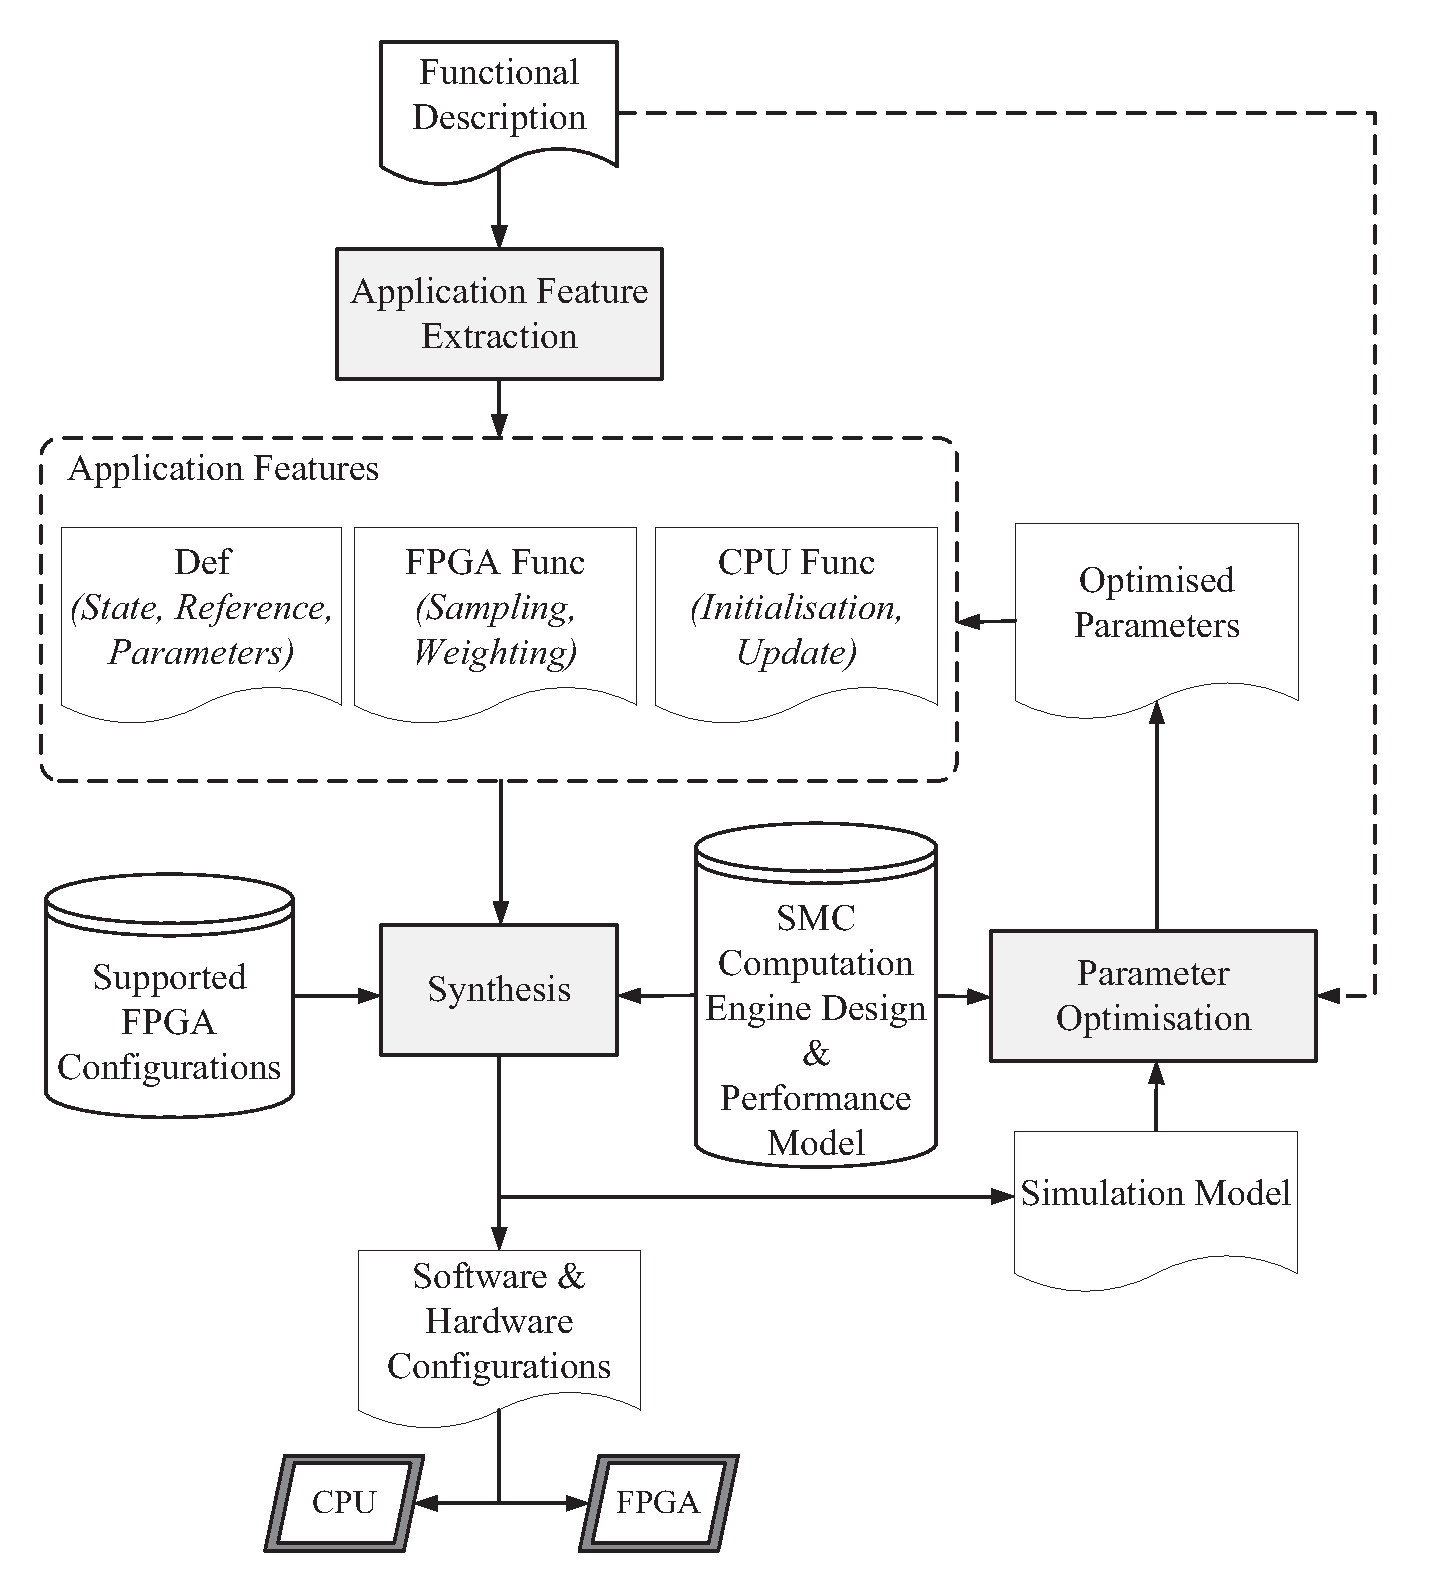
\includegraphics[width=0.6\textwidth]{design_flow/figures/flow}
\end{center}
\caption{Design flow for SMC applications. Users only customise the application-specific descriptions inside the dotted box.}
\label{fig:flow}
\end{figure}

Figure~\ref{fig:flow} shows the proposed design flow.
Starting with a functional specification such as software codes or mathematical descriptions, 
the users identify and code application-specific descriptions (Section~\ref{sec:kernel}). The design flow automatically weaves these descriptions with the computation engine (Section~\ref{sec:system}) to form a complete multiple-FPGA system.
In this work the synthesis tool employed is Maxeler's MaxCompiler, which uses Java as the underlying language. 
MaxCompiler also supports FPGAs from multiple vendors, such that low level configurations, such as I/O binding, are performed automatically.
Our approach can be extended to support other tools and devices, for example by having the appropriate templates in VHDL or Verilog.

\subsection{Specifying Application Features}
\label{sec:kernel}

Users create a new SMC design by customising the application-specific Java descriptions inside the dotted box of Figure~\ref{fig:flow}.
These descriptions correspond to \textit{Def} (Code~\ref{lst:def}), \textit{FPGA Func} (Code~\ref{lst:func}) and \textit{CPU Func}.

%\textbf{Def}: Recall from Section~\ref{sec:smc} that SMC is concerned with estimating state $s_t$ with the effect of control $c_t$. In the example application:
%\textit{state} is location ($x,y$) and heading $h$, and
%\textit{control} is the displacement $d$ and rotation $r$.
%Furthermore, \textit{design parameters} (Table~\ref{tab:parameters}) and application parameters need to be supplied.
\textbf{Def}: Code~\ref{lst:def} illustrates the class where number representation (floating-point, fixed-point with different bit-width), structs (state, reference), static parameters (Table~\ref{tab:parameters}) and system parameters are defined.
Users are allowed to customise number representation to benefit from the flexibility of FPGA and make trade-off between accuracy and design complexity.
State and reference structs determine the I/O interface.
Static parameters are defined in this class, while dynamic parameters are provided at run-time.
System parameters define device-specific properties such as clock speed and parallelism.
%Parameters are mapped to registers or ROMs in the FPGA.
%For certain applications, the set of parameters can be simplified, e.g.
%\textit{itl\_inner}, \textit{NA} and \textit{H} are set to 1 in this example.

\textbf{FPGA Func}: \textit{Sampling and importance weighting} (line~\ref{algo:s} and~\ref{algo:i} of Algorithm~\ref{algo:smc}) are the most computation intensive functions, and accelerated by FPGAs.
Code~\ref{lst:func} illustrates how these two FPGA functions are defined.
Given current state \textit{s\_in}, reference \textit{r\_in} and observation \textit{m\_in} (sensor values in this example), an estimation state \textit{s\_out} is computed.
Weight \textit{w} accounts for the probability of an observation from the estimated state.
The weight is calculated from the product of scores over the horizon.
In this example, the weight is equal to the score as the horizon length is only 1. 
%Constraints are then verified, i.e. if any elements of the state vector are negative, the weight is set to zero.

\textbf{CPU Func}: \textit{Initialisation and update} are functions running on the CPU.
They are responsible for obtaining and formatting data and displaying results.
\textit{resampling} is independent of applications so users need not to customise it.

\begin{Code}
    \centering
\lstset{language=Java,
        basicstyle=\ttfamily\small,
				tabsize=2,
				numbers=left,
				numberstyle=\tiny,
				frame=tb,
				columns=fullflexible,
				showstringspaces=false
				}
\begin{lstlisting}[][t!]
public class Def {
	// Number Representation
	static final DFEType float_t = 
		KernelLib.dfeFloat(8,24);
	static final DFEType fixed_t = 
		KernelLib.dfeFixOffset(26,-20,SignMode.TWOSCOMPLEMENT);
	// State Struct
	public static final DFEStructType state_t = new 
	DFEStructType(
		new StructFieldType(''x'', compType);
		new StructFieldType(''y'', compType);
		new StructFieldType(''h'', compType););
	// Reference Struct
	public static final DFEStructType ref_t = new 
	DFEStructType(
		new StructFieldType(''d'', compType);
		new StructFieldType(''r'', compType););
	// Static Design parameters (Table I)
	public static int NPMin = 5000, NPMax = 25000;
	public static int H = 1, NA = 1;
	// System Parameters
	public static int NC_inner = 1, NC_P = 2;
	public static int Clk_core = 120, Clk_mem = 350;
	public static int FPGA_resampling = 0, Use_DRAM = 0;
	// Application parameters
	public static int NWall = 8, NSensor = 20;
}
\end{lstlisting}
\caption{\small State, control and parameters for the robot localisation example.}
\label{lst:def}
\end{Code}

\begin{Code}
\centering
\lstset{language=Java,
        basicstyle=\ttfamily\small,
				tabsize=2,
				numbers=left,
				numberstyle=\tiny,
				frame=tb,
				columns=fullflexible,
				showstringspaces=false
				}
\begin{lstlisting}[][!t]
public class Func {
	public static DFEStruct sampling(
		DFEStruct s_in, DFEStruct c_in){
		DFEStruct s_out = state_t.newInstance(this);
		s_out.x = s_in.x + nrand(c_in.d,S*0.5) * cos(s_in.h);
		s_out.y = s_in.y + nrand(c_in.d,S*0.5) * sin(s_in.h);
		s_out.h = s_in.h + nrand(c_in.r,S*0.1);
		return s_out;
	}
	public static DFEVar weighting(
		DFEStruct s_in, DFEVar sensor){
		// Score calculation
		DFEVar score = exp(-1*pow(est(s_in)-sensor,2)/S/0.5);
		// Constraint handling
		bool succeed = est(s_in)>0 ? true : false;
		// Weight accumulation
		DFEVar w = succeed ? score : 0; //weight
		return w;
	}
}
\end{lstlisting}
\caption{\small FPGA functions (Sampling and importance weighting) for the robot localisation example.}
\label{lst:func}
\end{Code}


\subsection{Computation Engine Design}
\label{sec:system}

To allow customisation of the computation engine, the engine and data structure are designed as shown in Figure~\ref{fig:system} and~\ref{fig:stream} respectively.
The computation engine employs a heterogeneous structure that consists of multiple FPGAs and CPUs.
FPGAs are responsible for sampling, importance weighting and optionally resampling index generation, and fully pipelined to maximise throughput. 
To exploit parallelism, particle simulations (sampling and importance weighting) are computed simultaneously by every processing core on each FPGA. 
Processing cores can be replicated as many times as FPGA resources allow.
In situation where the computed results have to be grouped together, data are transferred among FPGAs via the inter-FPGA connection.
To maximise the system throughput, remaining non-compute-intensive tasks that involve random and non-sequential data accesses are performed on the CPUs.
FPGAs and CPUs communicate through high bandwidth connections such as PCI Express or InfiniBand.

\setcounter{subfigure}{0}
\begin{figure}[t!]
\centering
\subfigure[]{
	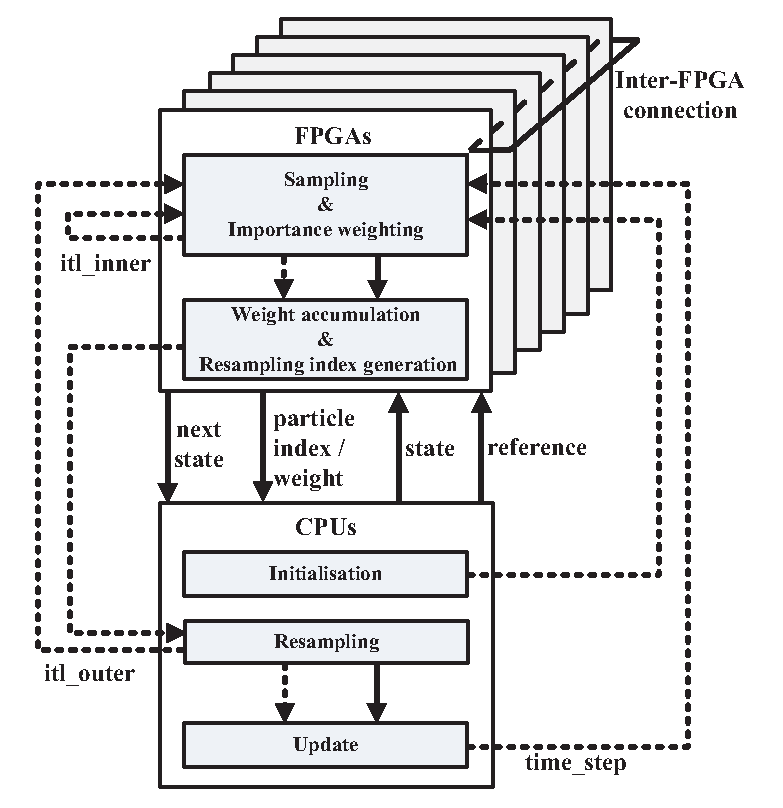
\includegraphics[width=0.7\textwidth]{design_flow/figures/system}
	\label{fig:system}
}
\subfigure[]{
	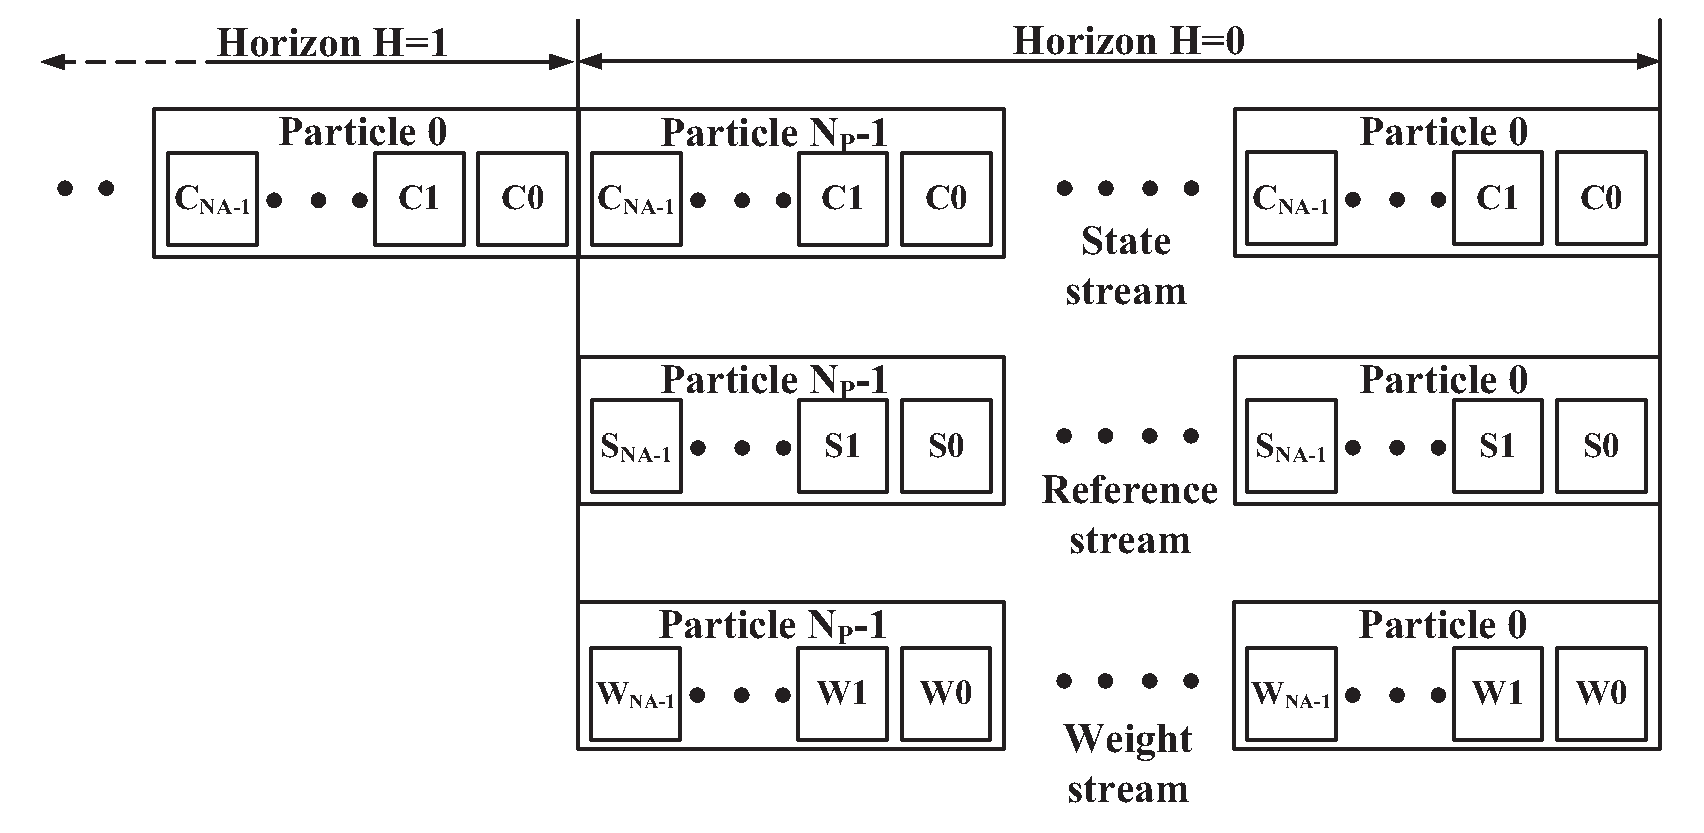
\includegraphics[width=0.8\textwidth]{design_flow/figures/stream}
	\label{fig:stream}
}
\caption{(a) Design of the SMC computation engine. Solid lines represent data paths while dotted lines represent control paths; (b) Data structure of particles represented by 3 data streams.}
\end{figure}

From the control paths (dotted lines) of Figure~\ref{fig:system}, we see that there are 3 loops matching Algorithm~\ref{algo:smc}: 
(1) inner, (2) outer, and (3) time step.
First, the inner loop iterates $itl\_inner$ number of times for \textit{sampling} and \textit{importance weighting},
$itl\_inner$ increases with the iteration count of the outer loop.
Second, the outer loop iterates $itl\_outer$ times to do \textit{resampling}.
The resampling process is performed $itl\_outer$ times to refine the pool of particles.
The particle indices are scrambled after this stage and the indices are transferred to the CPUs to update the particles.
Third, the time loop iterates once per time step to obtain a new control strategy and update the current state.

Based on this fact, the data structure shown in Figure~\ref{fig:stream} is derived.
%It utilises a deep pipeline of FPGAs so that particles can be processed simultaneously.
Each particle encapsulates 3 pieces of information: (1) state, (2) reference, and (3) weight, each being stored as a stream as indicated in the figure.
The length of the \textit{state stream} is $N_P \cdot N_A \cdot H$ because each control strategy predicts $H$ steps into the future.
The \textit{reference} and \textit{weight streams} have information of $N_A$ agents in $N_P$ particles.

Changing the values of $itl\_outer$, $itl\_inner$ and $N_P$ at run-time is allowed since they only affect the length of the particle streams, and not the hardware data path.
The computation engine is fully pipelined and outputs one result per clock cycle.

\begin{figure}[t!]
\begin{center}
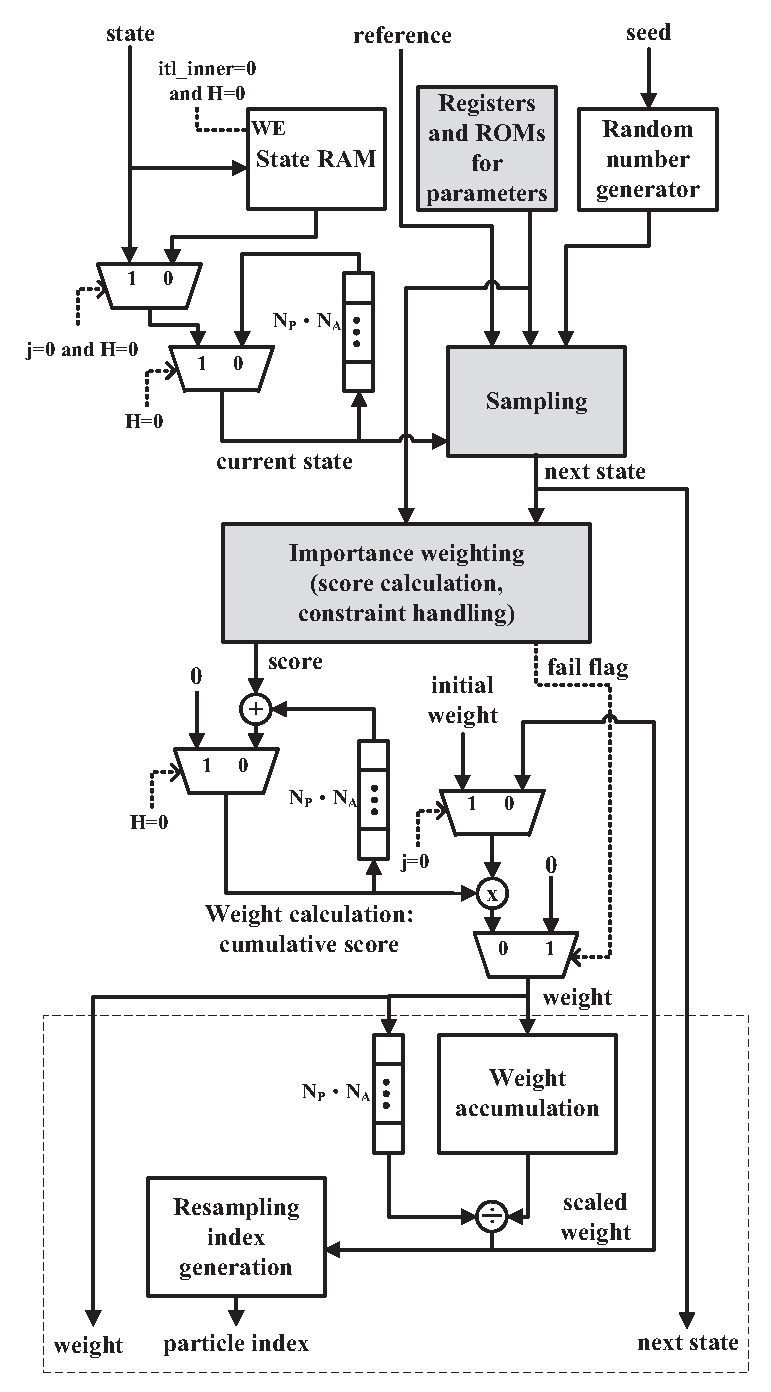
\includegraphics[width=0.6\textwidth]{design_flow/figures/kernel}
\end{center}
\caption{FPGA kernel design. The blocks that require users' customisation are darkened. The dotted box covers the blocks that are optional on FPGAs.}
\label{fig:kernel}
\end{figure}

Figure~\ref{fig:kernel} shows the design of the FPGA kernel. Blocks that require customisation are darkened.
The sampling function in Code~\ref{lst:func} is mapped to the \textbf{Sampling} block which accepts a state and a reference on each clock cycle and calculates the next state on the prediction horizon.
After getting a state from the CPU at the beginning ($itl\_inner=0$ and $H=0$), the data will be used by the kernel $itl\_inner \cdot N_P$ times.
An optional \textit{state RAM} enables reuse of state data and improve performance when the value of $itl\_inner$ is large.
An array of LUT-based random number generators~\cite{thomas07,thomas10} is seeded by CPU to provide random variables; application parameters are stored in registers; and
a feedback path stores the state of the previous $N_P \cdot N_A$ cycles.
%From this value, the next state on the horizon can be computed.

The \textbf{Importance weighting} block computes in 3 steps.
Firstly, \textit{Score calculation} uses the states from the \emph{Next state} block to calculate scores of all the states over the horizon.
A feedback loop of length $N_P \cdot N_A$ stores the cost of the previous horizon and accumulates the values.
Secondly, \textit{Constraint handling} uses the states from the \emph{Next state} block to check the constraints.
The block raises a fail flag if a constraint is violated.
Lastly, \textit{Weight calculation} combines the scores of the states over the horizon.

Part of the resampling process is handled by the \textbf{Resampling index generation} and \textbf{weight accumulation} blocks.
Weights are accumulated to calculate the cumulative distribution function, then particles indices are reordered.
These 2 blocks can either be computed on FPGAs or CPUs.

All the blocks allow precision customisation using fixed-point or floating-point number representation.
Users have the flexibility to make trade-off between result accuracy and design complexity.


\subsection{Performance Model}
\label{sec:model}

We derive a performance model to analyse the effect of parameters on the processing speed and resource utilisation of the computation engine.
It will be used in Section~\ref{sec:optimisation} for parameter optimisation.

The processing time of a time step is shown in Equation~\ref{eqt:time_step}.
It has 4 components which are iterated $itl\_outer$ times.

\begin{equation}
\footnotesize
\begin{aligned}
T_{step} = & itl\_outer \cdot \left (T_{s\&i} + T_{resample} + T_{cpu} + T_{transfer} \right)
\end{aligned}
\label{eqt:time_step}
\end{equation}
 
$T_{s\&i}$ is the time spent on sampling and importance weighting in the FPGA kernels.
Since the data is organised as a stream as described in Section~\ref{sec:system}, the time spent on sampling and importance weighting is linear with $N_P$, $N_A$ and $H$.
It is iterated $itl\_inner$ times in the inner loop.
The sampling and importance weighting process can be accelerated using multiple cores, such that each of them is responsible for part of the inner loop iterations or particles.
$N_C$ represents the number of processing cores being used on one FPGA, and $N_{Board}$ is the number of FPGA boards being used.
$min(1,\frac{bandwidth}{sizeof(state) \cdot freq})$ accounts for the limitation of bandwidth between FPGAs and CPUs.

\begin{equation}
\footnotesize
\begin{aligned}
T_{s\&i} = \frac{itl\_inner \cdot N_P \cdot N_A \cdot H}{N_C \cdot N_{Board} \cdot freq} \cdot \min\left(1,\frac{bandwidth}{sizeof(state) \cdot freq}\right)
\end{aligned}
\end{equation}

$T_{resample}$ is the time spent on generating the resampling indices.
It takes $N_P \cdot PW + N_P \cdot N_A$ cycles to generate the cumulative probability distribution function, and a further $3 \cdot PL \cdot N_P$ cycles to generate particle indices.
$PW$ and $PL$ are the length of the pipelines.
$T_{resample}$ can be omitted if resampling is processed by the CPUs.

\begin{equation}
\footnotesize
\begin{aligned}
T_{resample} = \frac{N_P \cdot PW + N_P \cdot N_A + 3 \cdot PL \cdot N_P}{freq}
\end{aligned}
\end{equation}

$T_{cpu}$ is the time spent on resampling and updating the current state on the CPUs.
The time is related to the amount of data and the speed of the CPU.
$\alpha_1$ is the scaling factor of the CPU speed.

\begin{equation}
\footnotesize
\begin{aligned}
T_{cpu} = \alpha_1 \cdot H \cdot N_P \cdot N_A
\end{aligned}
\end{equation}

$T_{transfer}$ is the data transfer time that accounts for the time taken to transfer the state stream between CPUs and DRAM on an FPGA board.
$T_{transfer}$ can be omitted if no DRAM is used.

\begin{equation}
\footnotesize
\begin{aligned}
T_{transfer} = \frac{N_P \cdot N_A \cdot \left ( H \cdot sizeof(state)\right)}{bandwidth}
\end{aligned}
\end{equation}

%Equation~\ref{eqt:usage_resource} shows the relation of logic, DSP and memory utilisation to parameters.
%$\beta_1, \beta_2, \beta_3, \beta_4, \beta_5$ are application specific parameters.
%The resource utilisations of logic, DSP and memory, denoted as $U_{logic}$, $U_{dsp}$ and $U_{mem}$ respectively, mainly scale with $N_A$.
%The usage of logic and memory is also affected by $N_P$ due to the use of feedback paths.
%$itl\_outer$ and $H$ affect the length of particles streams but not the resource usage.

%\begin{equation}
%\footnotesize
%\begin{aligned}
%U_{logic} & = \beta_1 N_A + \beta_2 N_P \\
%U_{dsp} & = \beta_3 N_A \\
%U_{mem} & = \beta_4 N_A + \beta_5 N_P 
%\end{aligned}
%\label{eqt:usage_resource}
%\end{equation}


%%%%%%%%%%%%%%%%%%%%%%%%%%%%%%%%%%%%%%%%%%%%%%%%%%%%%%%%%%%%%%%
\section{Optimising SMC Computation Engine}
\label{sec:optimisation}

The design parameters in Table~\ref{tab:parameters} have great impact on the performance.
3 questions manifest when finding optimised customisation of the engine:
\textbf{(1) Which sets of parameters have the best accuracy?
(2) For the same accuracy, which sets of parameters meet the timing requirement?
(3) How can we reduce the design parameter exploration time?}

\subsection{Effect of the Design Parameters}
\label{sec:parameters}

Referring to Table~\ref{tab:parameters}, the SMC computation engine has up to 6 design parameters, each of which adds a dimension to the design space.
It is ineffective to exhaustively search for the best set of parameters.
Furthermore, the performance curve of each dimension can be non-linear and constrained by the real-time requirement and FPGA resources.

To answer \textbf{questions 1 and 2}, consider the robot localisation application.
Its solution quality is measured by the root mean square error (RMSE) in localisation.
We study the effect of changing design parameters using the functional specification in Figure~\ref{fig:flow}, e.g. a C program.
Its fast build time helps us to perform analysis effectively but its performance is too slow for real-time operation.
The timing model described in Section~\ref{sec:model} estimates the run-time of the FPGA implementation.

When $N_P$ and $itl\_outer$ are explored together as shown in Figure~\ref{fig:mcl_2d}, we see an uneven surface.
Although non-linear, the trend of  RMSE decreasing as $N_P$ and $itl\_outer$ are increased is evident.
The valid parameter space is constrained by the real-time requirement.
The parameter space is darkened for those parameters leading to an RMSE greater than 1 m (Question 1).
Moreover, the dark region with a run-time longer than the 5 seconds real-time requirement is marked as invalid (Question 2).

\begin{figure}[t!]
\begin{center}
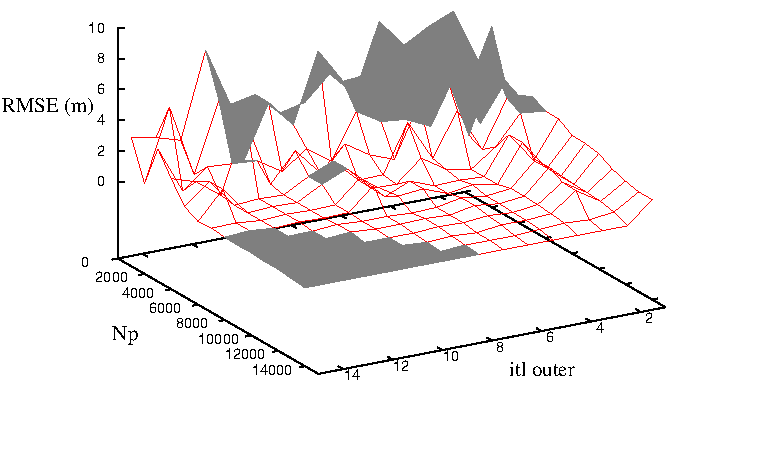
\includegraphics[width=0.8\textwidth]{design_flow/figures/fig_mcl_2d}
\end{center}
\caption{Parameter space of robot localisation system ($N_A$=8192, $S$=1). The dark region on the top-right indicates designs which fail localisation accuracy constraints, while those on the bottom-left indicates designs which fail real-time requirements.}
\label{fig:mcl_2d}
\end{figure}

If the value of $S$ is considered, the parameter optimisation problem expands to 3 dimensions as shown in Equation~\ref{eqt:opt_mcl}.
%In this application, $H=1$ and $itl\_inner=1$ so they are not explored.
%$U_{logic\_A}$, $U_{dsp\_A}$ and $U_{mem\_A}$ denote the resources available on the FPGA.

\begin{equation}
\footnotesize
\begin{aligned}
\mbox{minimise } RMSE &= f(N_P, itl\_outer, S) \\
\mbox{subject to } RMSE & \leq \mbox{1 m, } T_{step} \leq \mbox{5s, } \\
%U_{logic} \leq U_{logic\_A} \mbox{, } U_{dsp} & \leq U_{dsp\_A} \mbox{, } U_{mem} \leq U_{mem\_A} \\
\end{aligned}
\label{eqt:opt_mcl}
\end{equation}

%Next we look into \textbf{question 2}, minimising the run time so the robot can move more frequently.
%Although many sets of parameters produce the same solution quality, each set of parameters leads to very different run-time.
%The impact of the real-time constraint emerges in the dark region around the bottom left corner.
%It indicates that some parameter sets lead to designs with run-time exceeding the real-time requirement.


\subsection{Parameter Optimisation}
\label{sec:dse}

Now we come to \textbf{question 3}, the parameter optimisation problem, which is difficult as construction of an analytical model combining timing and quality of solution is either impossible or very time consuming. 
Furthermore the design space is constrained by multiple accuracy and real-time requirements.
We cannot use a design unless the results are within certain error bound.
The problem is further aggravated by the curse of dimensionality.
%We cannot assume that the general SMC methods parameters have the same impact on all applications which are based on SMC methods, the impact can be drastically different.
We use an automated design exploration approach which is facilitated by a machine learning algorithm developed in~\cite{kurek14}.
The approach allows the performance impact of different parameters to be determined for any design based on our SMC computation engine. 
%The approach has 4 steps:
%(1) Identify metrics to be optimised, such as RMSE and run-time.
%(2) Specify constraints that distinguish valid and invalid solutions.
%(3) Develop timing and resource models for the FPGA implementation.
%(4) Use the machine learning approach to explore the parameter space automatically.

A surrogate model is employed to enable rapid learning of the valid design space and deal with a large number of parameters.
%Regression of the fitness function is performed over the parameter space.
%An SVM classifier is used to prevent the algorithm from exploring regions of the parameter space which the classifier predicts to be invalid, i.e. they are likely to fail one of the constraints.
The idea is illustrated in Figure~\ref{fig:dse}.
Firstly, a number of randomly sampled designs is evaluated (Figure~\ref{fig:surrogate_sampling}).
Secondly, the results obtained during evaluations are used to build a surrogate model.
The model provides a regression of a fitness function and identifies regions of the parameter space which fail any of the constraints (Figure~\ref{fig:surrogate_regression}).
Thirdly, the surrogate model output is used to calculate the expected improvement (Figure~\ref{fig:surrogate_ei}).
Finally, the exploration converges to the parameter set that is expected to offer the highest improvement.
Parameter sets in the invalid region are disqualified (Figure~\ref{fig:surrogate_move}).

Our SMC computation engine is made customisable to improve productivity of application builders who target FPGAs, based on an optimisation approach which is already applicable to CPUs and GPUs. 

\setcounter{subfigure}{0}
\begin{figure}[t!]
\centering
\subfigure[]{
	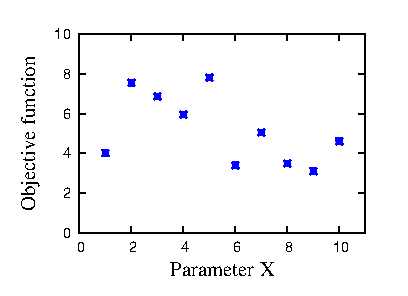
\includegraphics[width=0.4\textwidth]{design_flow/figures/fig_surrogate_sampling}
	\label{fig:surrogate_sampling}
}
\subfigure[]{
	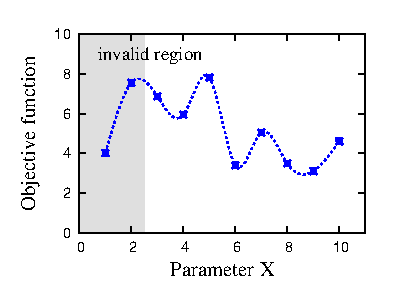
\includegraphics[width=0.4\textwidth]{design_flow/figures/fig_surrogate_regression}
	\label{fig:surrogate_regression}
}
\subfigure[]{
	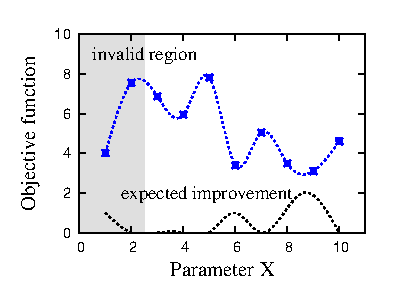
\includegraphics[width=0.4\textwidth]{design_flow/figures/fig_surrogate_ei}
	\label{fig:surrogate_ei}
}
\subfigure[]{
	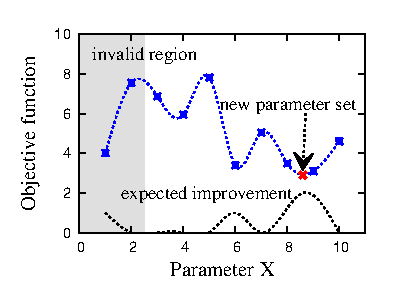
\includegraphics[width=0.4\textwidth]{design_flow/figures/fig_surrogate_move}
	\label{fig:surrogate_move}
}
\caption{Illustration of automatic parameter optimisation: (a) Sampling parameter sets; (b) Building surrogate model; (c) Calculating expected improvement; (d) Moving to the point offering the highest improvement.}
\label{fig:dse}
\end{figure}


%%%%%%%%%%%%%%%%%%%%%%%%%%%%%%%%%%%%%%%%%%%%%%%%%%%%%%%%%%%%%%%
\section{Evaluation}
\label{sec:evaluation}

%{\bf THOMAS - please comment on how the implementations were verified. Also comment on whether the chosen parameters were the same as the optimal ones (which can be found by exhaustive search).}

%3 applications are used to evaluate the design flow.

\subsection{Design Productivity}

We first analyse how the proposed design flow can reduce design effort.
In Table~\ref{tab:loc}, user-customisable code is classified into three parts:
(a) \textit{Def} is the definition of state, reference and parameters.
(b) \textit{FPGA Func} is the description of sampling and importance weighting functions.
(c) \textit{CPU Func} is the initiation, resampling and update part running on CPU.
On average, users only need to customise 24\% of the source code. 
Moreover, automatic design space optimisation greatly saves overall design time.
As we will see in the applications below, we are able to choose the optimal set of parameters without conducting an exhaustive search.
%While this is more difficult to quantify, we conservatively estimate the savings to be more than 50\% of the total design effort.

\begin{table}[h]
	\setlength{\tabcolsep}{3pt}
	\begin{spacing}{1.0}
	\caption{Lines of code for 3 SMC applications under the proposed design flow.}
	\label{tab:loc}
	\centering
	\smallskip
	\begin{threeparttable}
		\begin{tabular}{l|ccc|c|c}
			\hline
									& \multicolumn{3}{ |c| }{Custom codes} &  & \\
									\cline{2-4}
									& Def	& FPGA Func	& CPU Func & All codes	& Custom \% \\
			\hline
			\hline
			Sto. vol. 	& 31 & 44  & 84 & 1,164 & 13.7 \\
			Robot loc.	& 54 & 143 & 56 & 1,113 & 22.7 \\
			Air traffic	& 45 & 360 & 70 & 1,360 & 35.0 \\
			\hline
		\end{tabular}
	\end{threeparttable}
	\end{spacing}
\end{table}

\subsection{Application 1: Stochastic Volatility}

The stochastic volatility model was described using the flow 
Our design flow is used in targeting a stochastic volatility model to a XIlinx Virtex-6 XC6VSX475T FPGA at 150 MHz.
Parallel single precision floating-point data paths are used to maximise resource utilisation and hence performance.
Limited by I/O constraints, 16 processing cores are chosen. The resulting design uses 70,674 LUTs (24\%), 448 DSPs (22\%) and 394 block RAMs (19\%).
The CPU is an Intel Core i7 870 quad-core processor clocked at 2.93GHz.

The design space has 2 dimensions, $N_P$ and $S$ (Table~\ref{tab:parameters}).
Out of 420 sets of design parameters, the machine learning approach evaluates 20 of the candidates, and obtains an
optimal set of parameters $N_P=768, S=1.5$ which minimises the estimation error.

Table~\ref{tab:perf_sv} summarises the performance of CPU and reconfigurable systems using the same set of tuned parameters.
Both systems have the same microATX form factor for fair comparison.
Since the data size being processed is very small, the processing time of reconfigurable system is dominated by the overhead of invoking the FPGA kernel.

\begin{table}[h]
	\begin{spacing}{1.0}
	\caption{Performance comparison of stochastic volatility.}
	\label{tab:perf_sv}
	\centering
	\smallskip
	\begin{threeparttable}
		\begin{tabular}{l|x{2.2cm}y{2.2cm}}
			\hline
															& CPU~\tnote{a} 		& This work~\tnote{b} \\
			\hline
			\hline
			Clock frequency (MHz) 	& 2,930 	& 150  \\
			Number of cores					& 4				& 16 \\
			\hline
			\hline
			Run-time per step (ms) 	& 0.05		& 0.5 \\
			Power (W)								& 120			& 140 \\
			Energy (mJ)							&	6		& 70 \\
			\hline
		\end{tabular}
		\begin{tablenotes}
		\item[a] Intel Core i7 870 CPU, optimised by Intel Compiler with SSE4.2 and flag {\it -fast} enabled.
		\item[b] Maxeler MaxWorkstation with Xilinx Virtex-6 XC6VSX475T FPGA and Intel Core i7 870 CPU, developed using MaxCompiler.
		\end{tablenotes}
	\end{threeparttable}
	\end{spacing}
\end{table}

\subsection{Application 2: Mobile Robot Localisation}

Now we look at an application with larger data set.
For this example the same reconfigurable system as application 1 is used. 
Two processing cores are instantiated in an FPGA.
Core computation in the sampling and importance weighting process is implemented using fixed-point arithmetic to optimise resource usage.
The result utilises 148,431 LUTs (50\%), 1,278 DSPs (63\%) and 549 block RAMs (26\%).

The design space has 3 dimensions: $itl\_outer$, $N_P$ and $S$.
Out of 945 sets of parameters, 52 sets are evaluated to minimise the localisation error within the 5 seconds real-time constraint.

Table~\ref{tab:perf_mcl1} compares the performance of our reconfigurable system with CPU, GPU and a previous system in~\cite{chau13a} 
which has not been optimised by our proposed approach.
The reconfigurable system is 8.9 times and 1.2 times faster than the CPU and GPU, respectively.
With parameter optimisation that maximise accuracy, our work achieves a better RMSE than the previous work (0.15m vs. 0.52m).
%It is also the most energy efficient of all systems.

\begin{table}[h]
	\setlength{\tabcolsep}{2pt}
	\begin{spacing}{1.0}
	\caption{Performance comparison of robot localisation.}
	\label{tab:perf_mcl1}
	\centering
	\smallskip
	\begin{threeparttable}
		\begin{tabular}{l|x{3cm}y{3cm}x{3cm}x{3cm}}
			\hline
															& CPU 							& This work  				& Ref. sys.~\cite{chau13a}  	& GPU \\
															& opt.~\tnote{a}		&	opt.~\tnote{b}		& w/o opt.~\tnote{b}		& opt. ~\tnote{c} \\
			\hline
			\hline
			Clk. freq. (MHz) 	& 2,930 & 120 	& 100 	& 1,150 \\
			Number of cores					& 4		& 2 	& 2 	& 448 \\
			\hline
			\hline
			Run-time / step (s) 	& 33.1	& 3.7	& 1.6			& 4.5 \\
			RMSE (m)								& 0.15	& 0.15	& 0.52	& 0.15 \\
			Power (W)								& 130		& 145 	& 145		& 287 \\
			Energy (kJ)							& 4.3		& 0.54	& 0.23	& 1.29 \\
			\hline
		\end{tabular}
		\begin{tablenotes}
		\item[a,b] Refer to configurations in Table~\ref{tab:perf_sv}.
		\item[c] NVIDIA Tesla C2070 GPU, developed using CUDA programming model.
		\item[d] Parameters with optimisation: $itl\_outer$=2, $N_P$=14000, $S$=1.2; \\ Parameters without optimisation: $itl\_outer$=1, $N_P$=8192, $S$=1. 
		\end{tablenotes}
	\end{threeparttable}
	\end{spacing}
\end{table}

\subsection{Application 3: Air Traffic Management}

The air traffic management system is able to control 20 aircraft simultaneously.
The FPGA part runs on a 1U machine hosting 6 Altera Stratix V GS 5SGSD8 FPGAs clocked at 220 MHz, 
each of which has a single precision floating-point data path that consumes 166,008 LUTs (63\%), 337 multipliers (9\%) and 1,528 block RAMs (60\%).
The CPU part runs on 2 Intel Xeon E5-2640 CPUs clocked at 2.53GHz.
Both parts are connected via InfiniBand.

This application has 4 design parameters leading to a space with 4000 sets of parameters.
The optimisation target is to minimise the time of aircraft spending in the air traffic control region.
Machine learning reduces the number of evaluations to 1\% as indicated in Table~\ref{tab:dse}.
Hence, the parameter optimisation time is reduced from days to hours.

\begin{table}[h]
	\begin{spacing}{1.0}
	\caption{Parameter optimisation of air traffic management system using machine learning approach.}
	\label{tab:dse}
	\centering
	\smallskip
	\begin{threeparttable}
		\begin{tabular}{l|c|c c c c}
			\hline
			\multirow{2}{*}{$N_A$}			& Parameter	sets		& \multicolumn{4}{|c}{Parameter set obtained} \\
			\cline{3-6}
																	& evaluated / total					& $itl\_outer$  		& $H$ & $N_P$ & $S$ \\
			\hline
			\hline
			4 													& 41 / 4000											& 20								&	5		&	500	  & 0.1 \\
			%12 													& 39 / 4000 											& 20								&	5		&	1000	& 0.05 \\
			20													& 31 / 4000 											& 100								&	8		&	5000	& 0.05 \\
			\hline
		\end{tabular}
	\end{threeparttable}
	\end{spacing}
\end{table}

\begin{table}[ht]
	\setlength{\tabcolsep}{3pt}
	\begin{spacing}{1.0}
	\caption{Performance comparison of air traffic management.}
	\label{tab:perf_comparison}
	\centering
	\smallskip
	\begin{threeparttable}
		\begin{tabular}{c|p{4cm}|ccgc}
			\hline
															&											& CPU										& GPU 									& This work 					& Ref. FPGA~\cite{chau13b} 	\\
															&											& opt.~\tnote{a}		& opt.~\tnote{b} 	& opt.~\tnote{c} & w/o opt.~\tnote{d} 	\\
			\hline
			\hline
															& Clk. freq. (MHz) & 2,660 							& 1,150 								& 220 								& 150  \\
															& Number of cores			& 24										& 1,792									& 6										& 5 \\
															& Power (W)						& 550										& 1100									& 600									& N/A \\
			\hline
			\hline
			4												& Run-time / step (s)	& 0.80		 			&	0.12									&	0.03								& 2.2 \\
			aircraft								& Energy (kJ)					& 0.44									& 0.13									& 0.02								& N/A \\
			\hline
			20											& Run-time / step (s)	& 198	 					&	28.25									&	11.6								& N/A \\
			aircraft								& Energy (kJ)					& 108.90								& 29.95									& 7.0									& N/A \\
			\hline
		\end{tabular}
		\begin{tablenotes}
		\item[a] 4 Intel Xeon X5650 CPUs (scaled), optimised by Intel Compiler with SSE4.2 and flag {\it -fast} enabled.
		\item[b] 4 NVIDIA Tesla C2070 GPUs (scaled), developed using CUDA programming model.
		\item[c] Maxeler MPC-X2000, with 6 Altera Stratix V GS 5SGSD8 FPGAs and 2 Intel Xeon X5650 CPUs, developed using MaxCompiler.
		\item[d] Altera Stratix IV EP4SGX530 FPGA.
		\item[e] Parameters with optimisation: refer to Table~\ref{tab:dse};\\ Parameters without optimisation: $itl\_outer$=100, $N_P$=1024, $S$=0.05, $H$=6.
		\end{tablenotes}
	\end{threeparttable}
	\end{spacing}
\end{table}

Table~\ref{tab:perf_comparison} summarises the performance of the CPU, GPU and reconfigurable system.
To ensure fair comparisons, we scale the CPU and GPU systems to similar form factors with the reconfigurable system.
The scaling is based on the fact that the sampling and importance weighting process is evenly distributed to every GPU and computed independently,
while the resampling process is computed on the CPU no matter how many GPUs are used.
The reconfigurable platform is faster and more energy efficient than the other systems.

We also compare the performance of our work with a reference implementation that uses an Altera Stratix IV FPGA~\cite{chau13b}.
That implementation is only large enough to support 4 aircraft and it does not have the flexibility to tune parameters without re-compilation.
Our design exploration approach is able to select the set of parameters that produces the same quality of results and is up to 73 times faster.

%Our SMC computation engine is also easily scalable.
%For example, in a future scenario with 50 aircraft and a reconfigurable platform with 24 FPGAs, design exploration indicates that
%we could change the parameter setting to $itl\_outer=120$, $H=10$, $N_P=8000$ and still meet the real-time requirement without any hardware redesign.


%%%%%%%%%%%%%%%%%%%%%%%%%%%%%%%%%%%%%%%%%%%%%%%%%%%%%%%%%%%%%%%
\section{Summary}
\label{sec:summary}

This paper demonstrates the feasibility of generating highly-optimised reconfigurable designs for SMC applications, while hiding detailed implementation aspects from the user.  
A software template makes the computation engine portable and facilitates code reuse, the number of lines of user-written code being decreased by approximately 76\% for an application.
We further establish that a surrogate software model combined with machine learning can be used to rapidly optimise designs, reducing optimisation time from days to hours; 
and that the resulting parameters can be utilised without resynthesis. 
%For the stochastic volatility, robot localisation and air traffic management examples explored, the resulting designs improved on the previously best reported implementations.

Ongoing and future work is focused on incorporating device-specific parameters, such as the level of parallelism and clock speed, into the machine learning approach~\cite{kurek14}.
We are currently investigating run-time optimisation of parameters based on our initial work ~\cite{chau13a}.
We will also automate the design flow to allow translation of designs captured in software programming languages (e.g. R, MATLAB) to reconfigurable implementations,
and extend the software template in VHDL/Verilog to support a wider range of systems.
%We are currently applying this work to cover more SMC applications, 
%including aerial vehicle (UAV)~\cite{conde09} navigation 
%where real-time performance and lower energy consumption are major design considerations.

